\begin{lstlisting}
第三章 11 12 14 15 17 18
\end{lstlisting}
\begin{figure}[H]
\centering
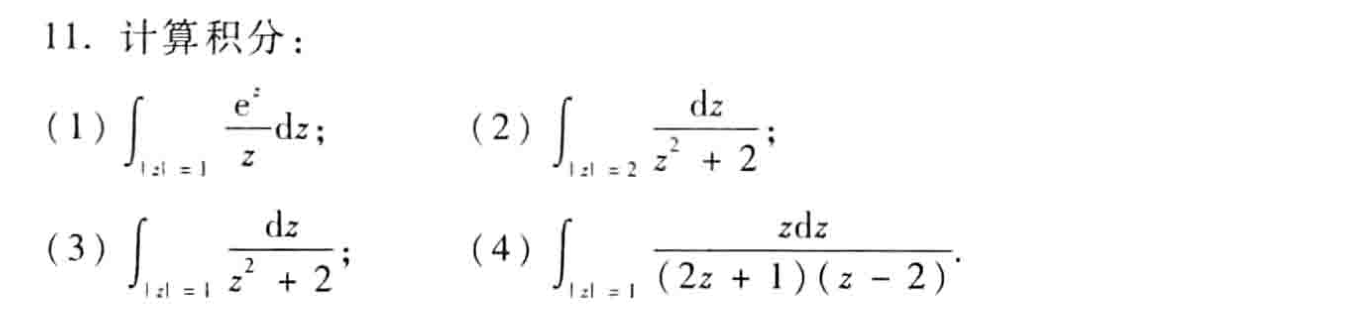
\includegraphics[width=\textwidth]{hw6-2025040513.png}
% \caption{}
\label{}
\end{figure}

(1)
\[
\int_{\lvert z \rvert =1}^{} \frac{e^{ z }}{z} \, dz \overset{ Cauchy }{ = }2\pi i\left.(e^{ z })\right|_{z=0}=2\pi i
\]
(2)
\[
\int_{\lvert z \rvert =2}^{} \frac{1}{z^2+2}  \, \mathrm{d}z =\frac{1}{2\sqrt{ 2 }i} \int_{\lvert z \rvert =2}^{}\left(  \frac{1}{z-\sqrt{ 2 }i} -\frac{1}{z+\sqrt{ 2 }i} \right)  \, \mathrm{d}z =0
\]
(3)
Since $\frac{1}{z^2+2}$ is holomorphic in the unit disc and its boundary,
\[
\int_{\lvert z \rvert =1}^{} \frac{1}{z^2+2}  \, \mathrm{d}z= 0
\]
(4)
\[
\int_{\lvert z \rvert =1}^{} \frac{z}{(2z+1)(z-2)} \, \mathrm{d}z=2\pi i\left( \frac{z}{2(z-2)}  \right)_{z=-1/2 }=\frac{\pi i}{5}
\]
\begin{figure}[H]
\centering
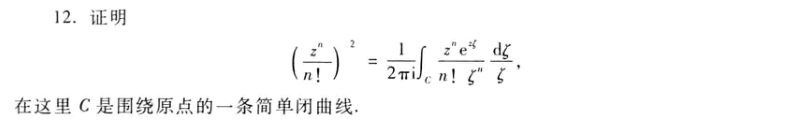
\includegraphics[width=\textwidth]{hw6-2025040411.png}
% \caption{}
\label{}
\end{figure}

Apply Cauchy's integral formula to $f(\eta)=e^{ z \eta }$ at $\eta=0$, then
\[
z^{n}=f^{(n)}(0)=\frac{n!}{2\pi i}\int_{C}^{} \frac{e^{ z \zeta }}{\zeta^{n}} \, d\zeta 
\]
Therefore
\[
\left( \frac{z^{n}}{n!} \right)^{2}=\frac{1}{2\pi i}\int_{C}^{} \frac{z^{n}}{n!}\cdot\frac{e^{ z\zeta }}{\zeta^{n}} \, d\zeta
\]
\begin{figure}[H]
\centering
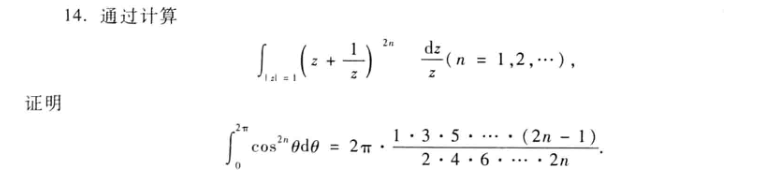
\includegraphics[width=\textwidth]{1-hw6-2025040411.png}
% \caption{}
\label{}
\end{figure}
\[
\int_{\lvert z \rvert =1}^{} \left( z+\frac{1}{z} \right)^{2n}\cdot\frac{1}{z}  \, dz   =\int_{\lvert z \rvert=1 }^{} \frac{(z^2+1)^{2n}\cdot z^{-n}}{z^{n+1}} \, dz 
\]
Let
\[
f(z)\coloneqq (z^2+1)^{2n}\cdot z^{-n}=\sum_{k=0}^{2n} C^{k}_{2n}z^{2k-n}
\]
Then
\[
f^{(n)}(z)=\sum_{k=0}^{2n} C^{k}_{2n}\cdot(2k-n)\dots(2k-2n+1)\cdot z^{2k-2n}
\]
Let $z=0$ then
\[
f^{(n)}(0)=C^{n}_{2n}\cdot n!
\]
Thus
\[
\int_{\lvert z \rvert =1}^{} \left( z+\frac{1}{z} \right)^{2n}\cdot\frac{1}{z} \, dz=\int_{\lvert z \rvert =1}^{} \frac{f(z)}{z^{n+1}} \, dz=  \frac{2\pi i}{n!}f^{(n)}(0)=2\pi i\cdot\frac{(2n)!}{n!\cdot n!}
\]
On the other hand
\[
\int_{\lvert z \rvert =1}^{} \left( z+\frac{1}{z} \right)^{2n}\cdot\frac{1}{z} \, dz=\int_{0}^{2\pi} (e^{ i\theta }+e^{ -i\theta })^{2n}\cdot i \, d\theta=i\cdot\int_{0}^{2\pi} 2^{2n}\cdot \cos ^{2n}\theta \, d\theta
\]
Therefore
\[
\int_{0}^{2\pi} \cos ^{2n}\theta \, d\theta=2\pi \cdot\frac{(2n-1)!!}{(2n)!!}
\]
\begin{figure}[H]
\centering
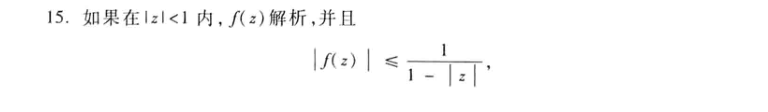
\includegraphics[width=\textwidth]{2-hw6-2025040411.png}
% \caption{}
\label{}
\end{figure}
\begin{figure}[H]
\centering
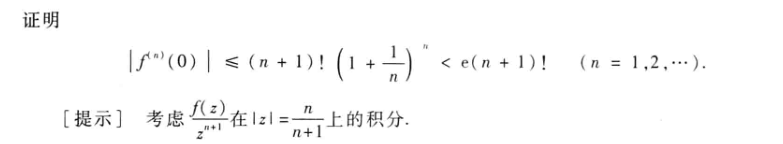
\includegraphics[width=\textwidth]{3-hw6-2025040411.png}
% \caption{}
\label{}
\end{figure}

For $0<r<1$, apply the Cauchy's integral formula
\[
\lvert f^{(n)}(0) \rvert =\left\lvert  \frac{n!}{2\pi i} \int_{\lvert z \rvert =r}^{} \frac{\lvert f(\zeta) \rvert }{\zeta^{n+1}}  \, d\zeta  \right\rvert \leq \frac{n!}{2\pi}\cdot\frac{2\pi r}{(1-r)r^{n+1}}  =\frac{n!}{(1-r)r^{n}}
\]
Clearly, $g(r)=(1-r)r^{n}$ reaches its maximum at $r=\frac{n}{n+1}$. Let $r=\frac{n}{n+1}<1$ then
\[
\lvert f^{(n)}(0) \rvert \leq (n+1)!\cdot\left( 1+\frac{1}{n}  \right)^{n}<e\cdot(n+1)!
\]
\begin{figure}[H]
\centering
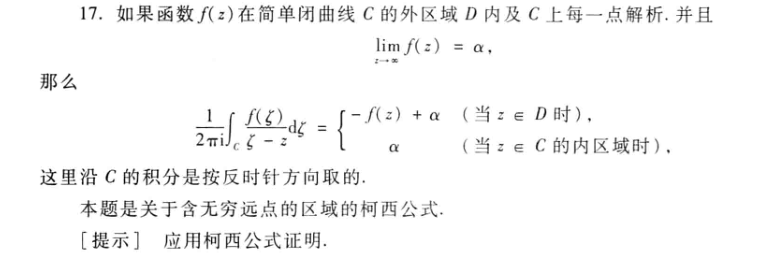
\includegraphics[width=\textwidth]{4-hw6-2025040411.png}
% \caption{}
\label{}
\end{figure}

When $z\in C^{\circ}$,

Let $R$ large enough such that $C$ is contained in $C_{R}$, where $C_{R}$ is the circle centered at $z$ with radius $R$, counterclockwise. Then
\[
\frac{1}{2\pi i}\int_{C}^{} \frac{f(\zeta)}{\zeta-z} \, d\zeta=\frac{1}{2\pi i}  \int_{C_{R}}^{} \frac{f(\zeta)}{\zeta-z} \, d\zeta
\]
$\forall \epsilon>0$, $\exists A>0$ s.t. $\forall \lvert z \rvert>A$, we have
\[
\lvert f(z)-\alpha \rvert<\epsilon
\]
Then for $R>A$
\[
\left\lvert  \frac{1}{2\pi i} \int_{C_{R}}^{} \frac{f(\zeta)}{\zeta-z} \, d\zeta-\alpha  \right\rvert =\left\lvert  \frac{1}{2\pi i} \int_{C_{R}}^{} \frac{f(\zeta)-\alpha}{\zeta-z} \, d\zeta  \right\rvert \leq \frac{\epsilon}{2\pi} \int_{C_{R}}^{} \frac{1}{\underbrace{ \lvert \zeta-z \rvert  }_{ =R }}  \, d\zeta= \epsilon
\]
Thus
\[
\left\lvert  \frac{1}{2\pi i}\int_{C}^{} \frac{f(\zeta)}{\zeta-z} \, d\zeta -\alpha  \right\rvert \leq \epsilon
\]
Since $\epsilon$ is arbitrary,
\[
\frac{1}{2\pi i}\int_{C}^{} \frac{f(\zeta)}{\zeta-z} \, d\zeta=\alpha  
\]
When $z\in D$, let $C_{\epsilon}$ be the circle centered at $z$ with radius $\epsilon$, clockwise. $\epsilon$ is small enough such that $C_{\epsilon}$ is contained in $D$. Then
\[
\frac{1}{2\pi i}\left( -\int_{C}^{} +\int_{C_{R}}+\int_{C_{\epsilon}} \right) \frac{f(\zeta)}{\zeta-z} \, d\zeta  =0
\]
By Cauchy's integral formula
\[
\frac{1}{2\pi i}\int_{C_{\epsilon}}^{} \frac{f(\zeta)}{\zeta-z} \, d\zeta=-2\pi if(z)
\]
Hence
\[
\frac{1}{2\pi i}\int_{C}^{} \frac{f(\zeta)}{\zeta-z} \, d\zeta=-f(z)+\alpha
\]
\begin{figure}[H]
\centering
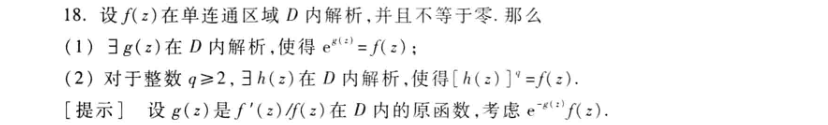
\includegraphics[width=\textwidth]{5-hw6-2025040411.png}
% \caption{}
\label{}
\end{figure}

(1)
Fix a point $z_0\in D$ and define
\[
g(z)=\int_{\gamma}^{} \frac{f'(w)}{f(w)}  \, dw+c_0
\]
where $\gamma$ is any path in $D$ connecting $z_0$ to $z$ and $c_0$ is a complex number so that $e^{ c_0 }=f(z_0)$. This definition is independent of the path $\gamma$ since $D$ is simple connected. We find that $g$ is holomorphic with
\[
g'(z)=\frac{f'(z)}{f(z)}
\]
and a simple calculation gives
\[
\frac{d}{dz}(f(z)e^{ -g(z) })=0
\]
so that $f(z)e^{ -g(z) }$ is constant. Evaluating this expression at $z_0$ we find $f(z_0)e^{ -g(z_0) }=1$ so that $f (z)=e^{ g (z) }$ for all $z\in D$, and the proof is complete.

(2)

(1) implies (2). Put $h(z)=e^{ \frac{1}{q}g(z) }$, then $h^{q}(z)=e^{ g(z) }=f(z)$.
